Dans cette section, nous présentons et analysons les résultats de nos simulations sur la propagation des défauts dans les réseaux financiers d'Erdös-Rényi.

\subsection{Observation d'un seuil critique dans la propagation des défauts}\label{subsec:observation-d'un-seuil-critique-dans-la-propagation-des-defauts}

Nos simulations mettent en évidence un phénomène intéressant à analyser : lorsque l'amplitude du choc atteint environ 50\% de la valeur totale des actifs extérieurs du système ($S \approx 0.5 \times \sum(c_i)$), on observe une augmentation significative du taux de défaut dans le réseau.
Ce seuil semble persister pour différentes tailles de réseau et différentes densités de connexion, comme l'illustre la Figure~\ref{fig:default_vs_shock}.

\begin{figure}[htbp]
    \centering
    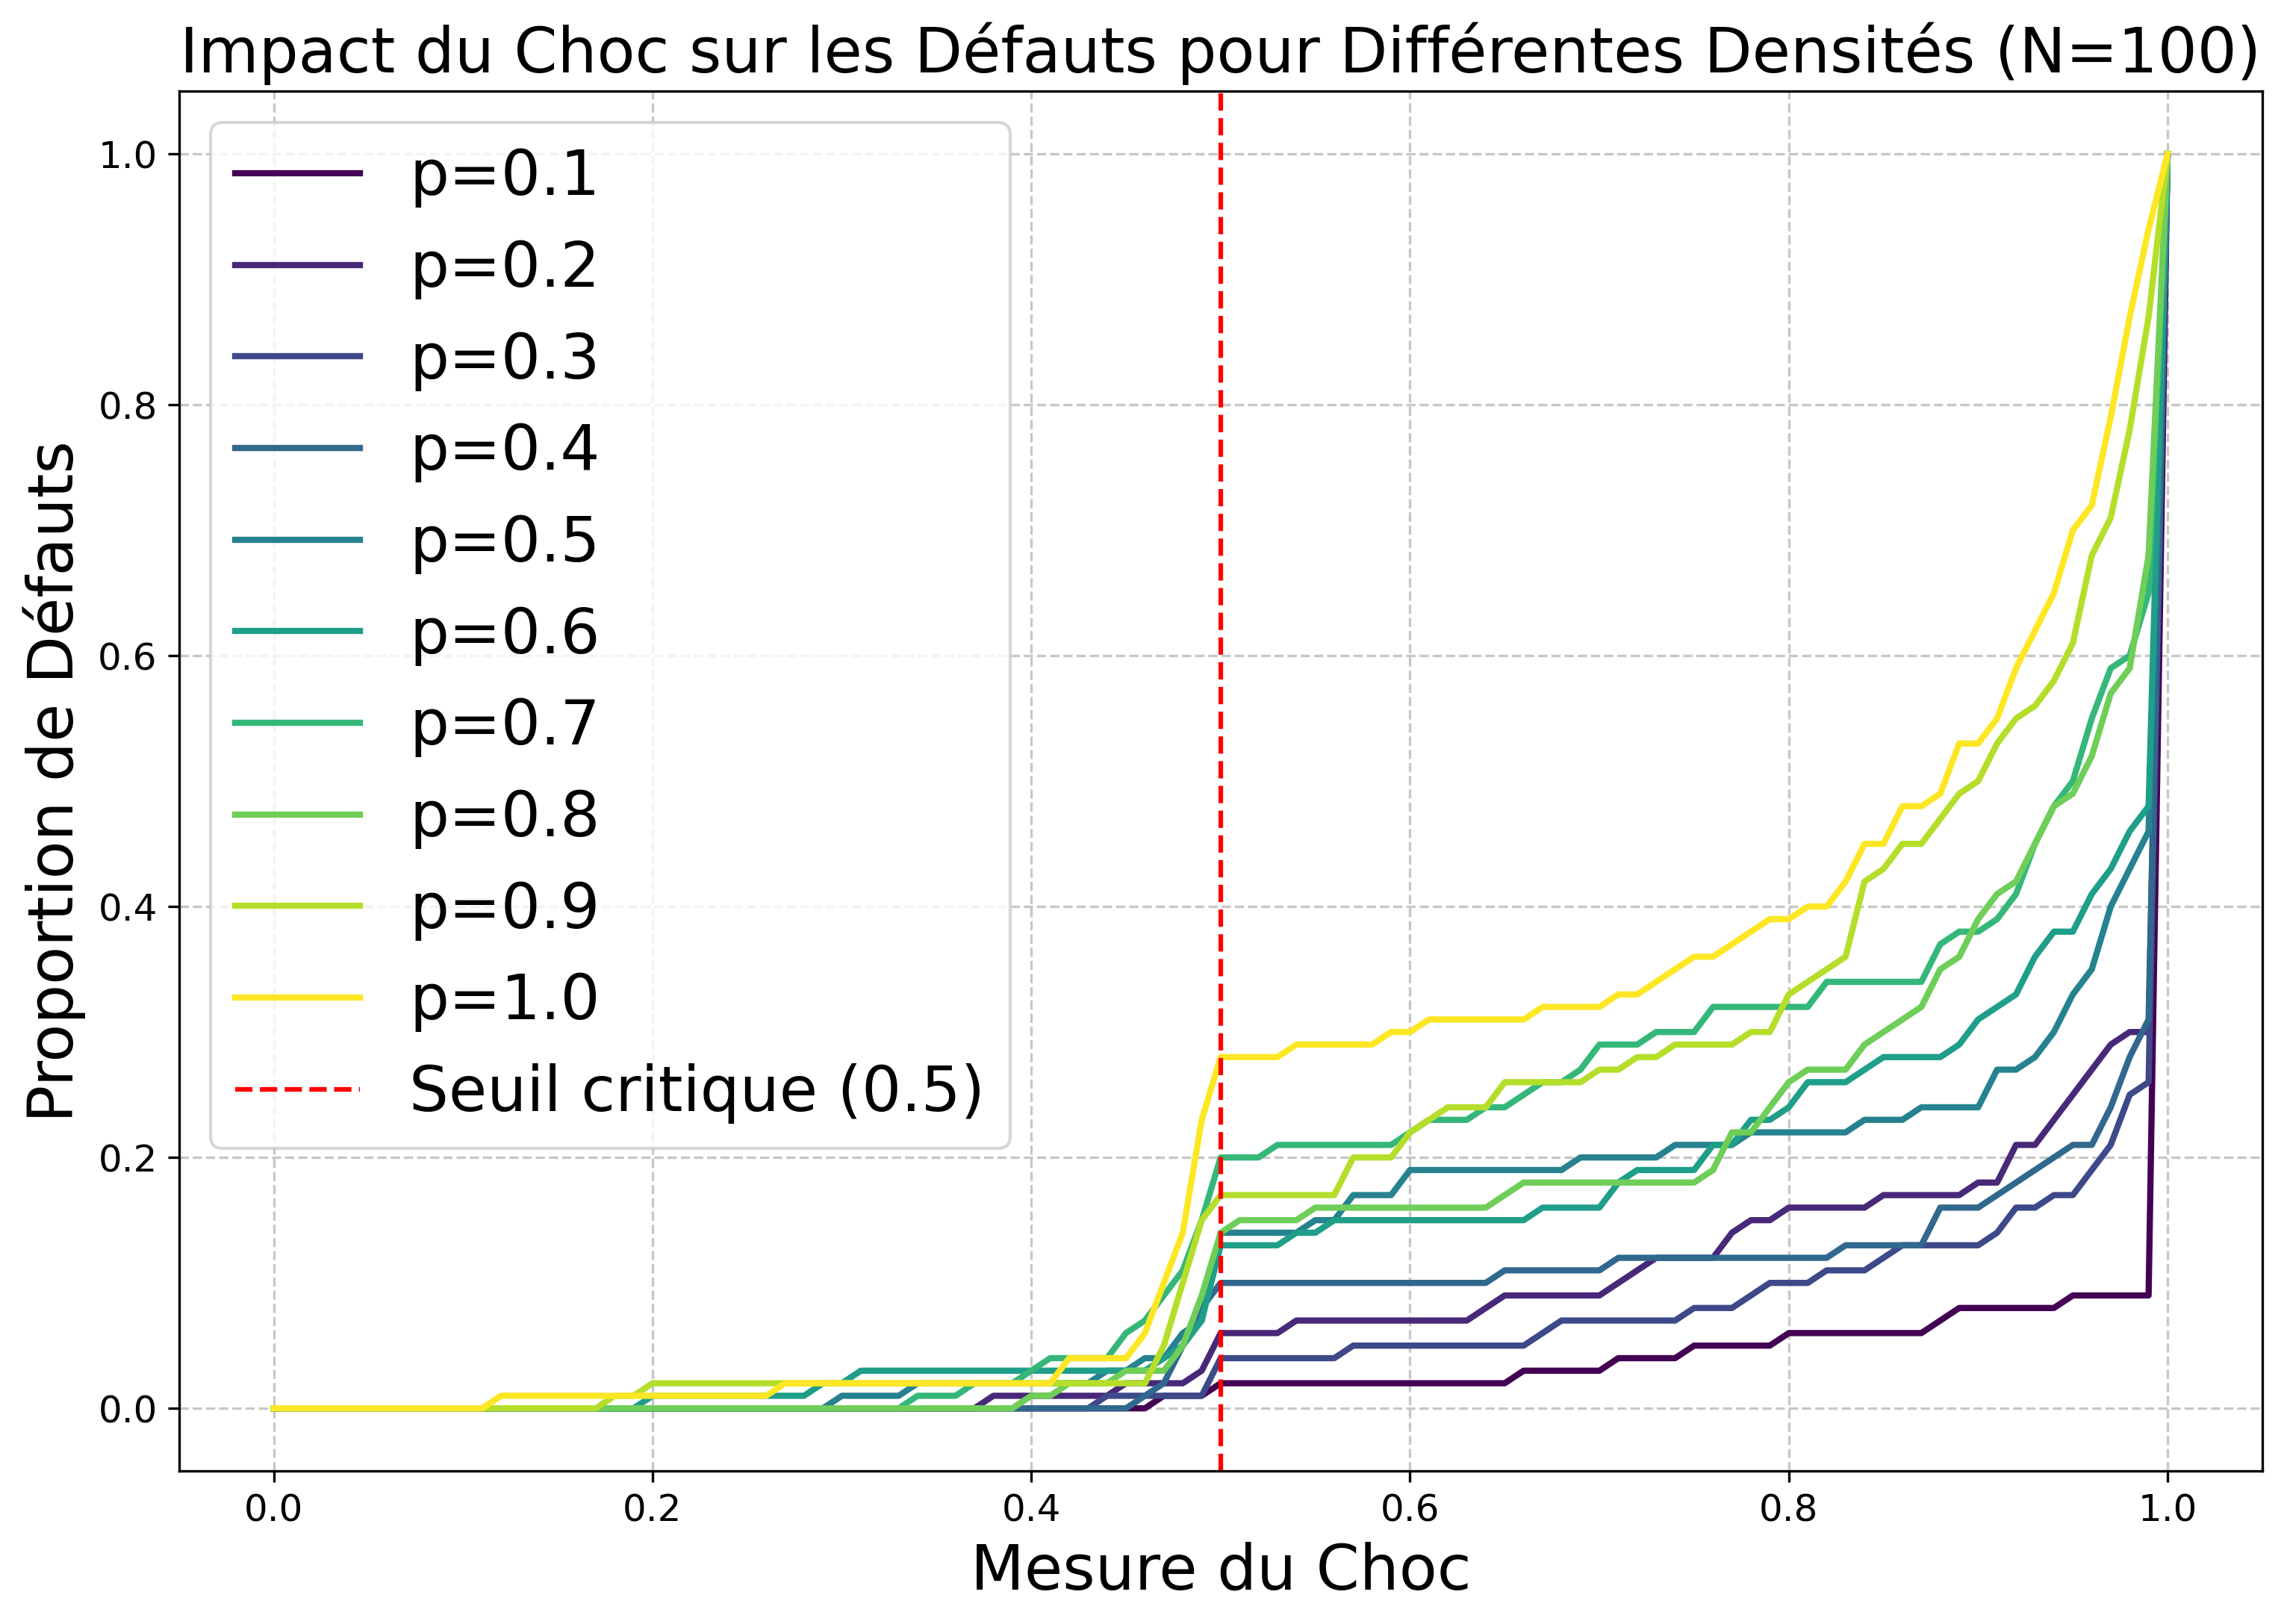
\includegraphics[width=\columnwidth]{fig2_2d_prob_shock_default.png}
    \caption{Proportion de défauts en fonction de la mesure du choc pour différentes probabilités de connexion dans un réseau de 100 banques.}
    \label{fig:default_vs_shock}
\end{figure}

Cette observation se caractérise par trois aspects principaux :
\begin{enumerate}
    \item Une augmentation notable de la proportion de défauts autour de ce seuil
    \item Un pic dans la dérivée de la courbe de défauts à ce point spécifique, visible dans la Figure \ref{fig:variation_default}
    \item Une relative stabilisation après ce pic, suggérant un changement de régime dans la dynamique de propagation
\end{enumerate}
De plus, ces courbes reflètent bien ce qu'on attend intuitevement lorsque la mesure de choc croit de manière linéaire, la proportion de défaut augmente également.

\begin{figure}[htbp]
    \centering
    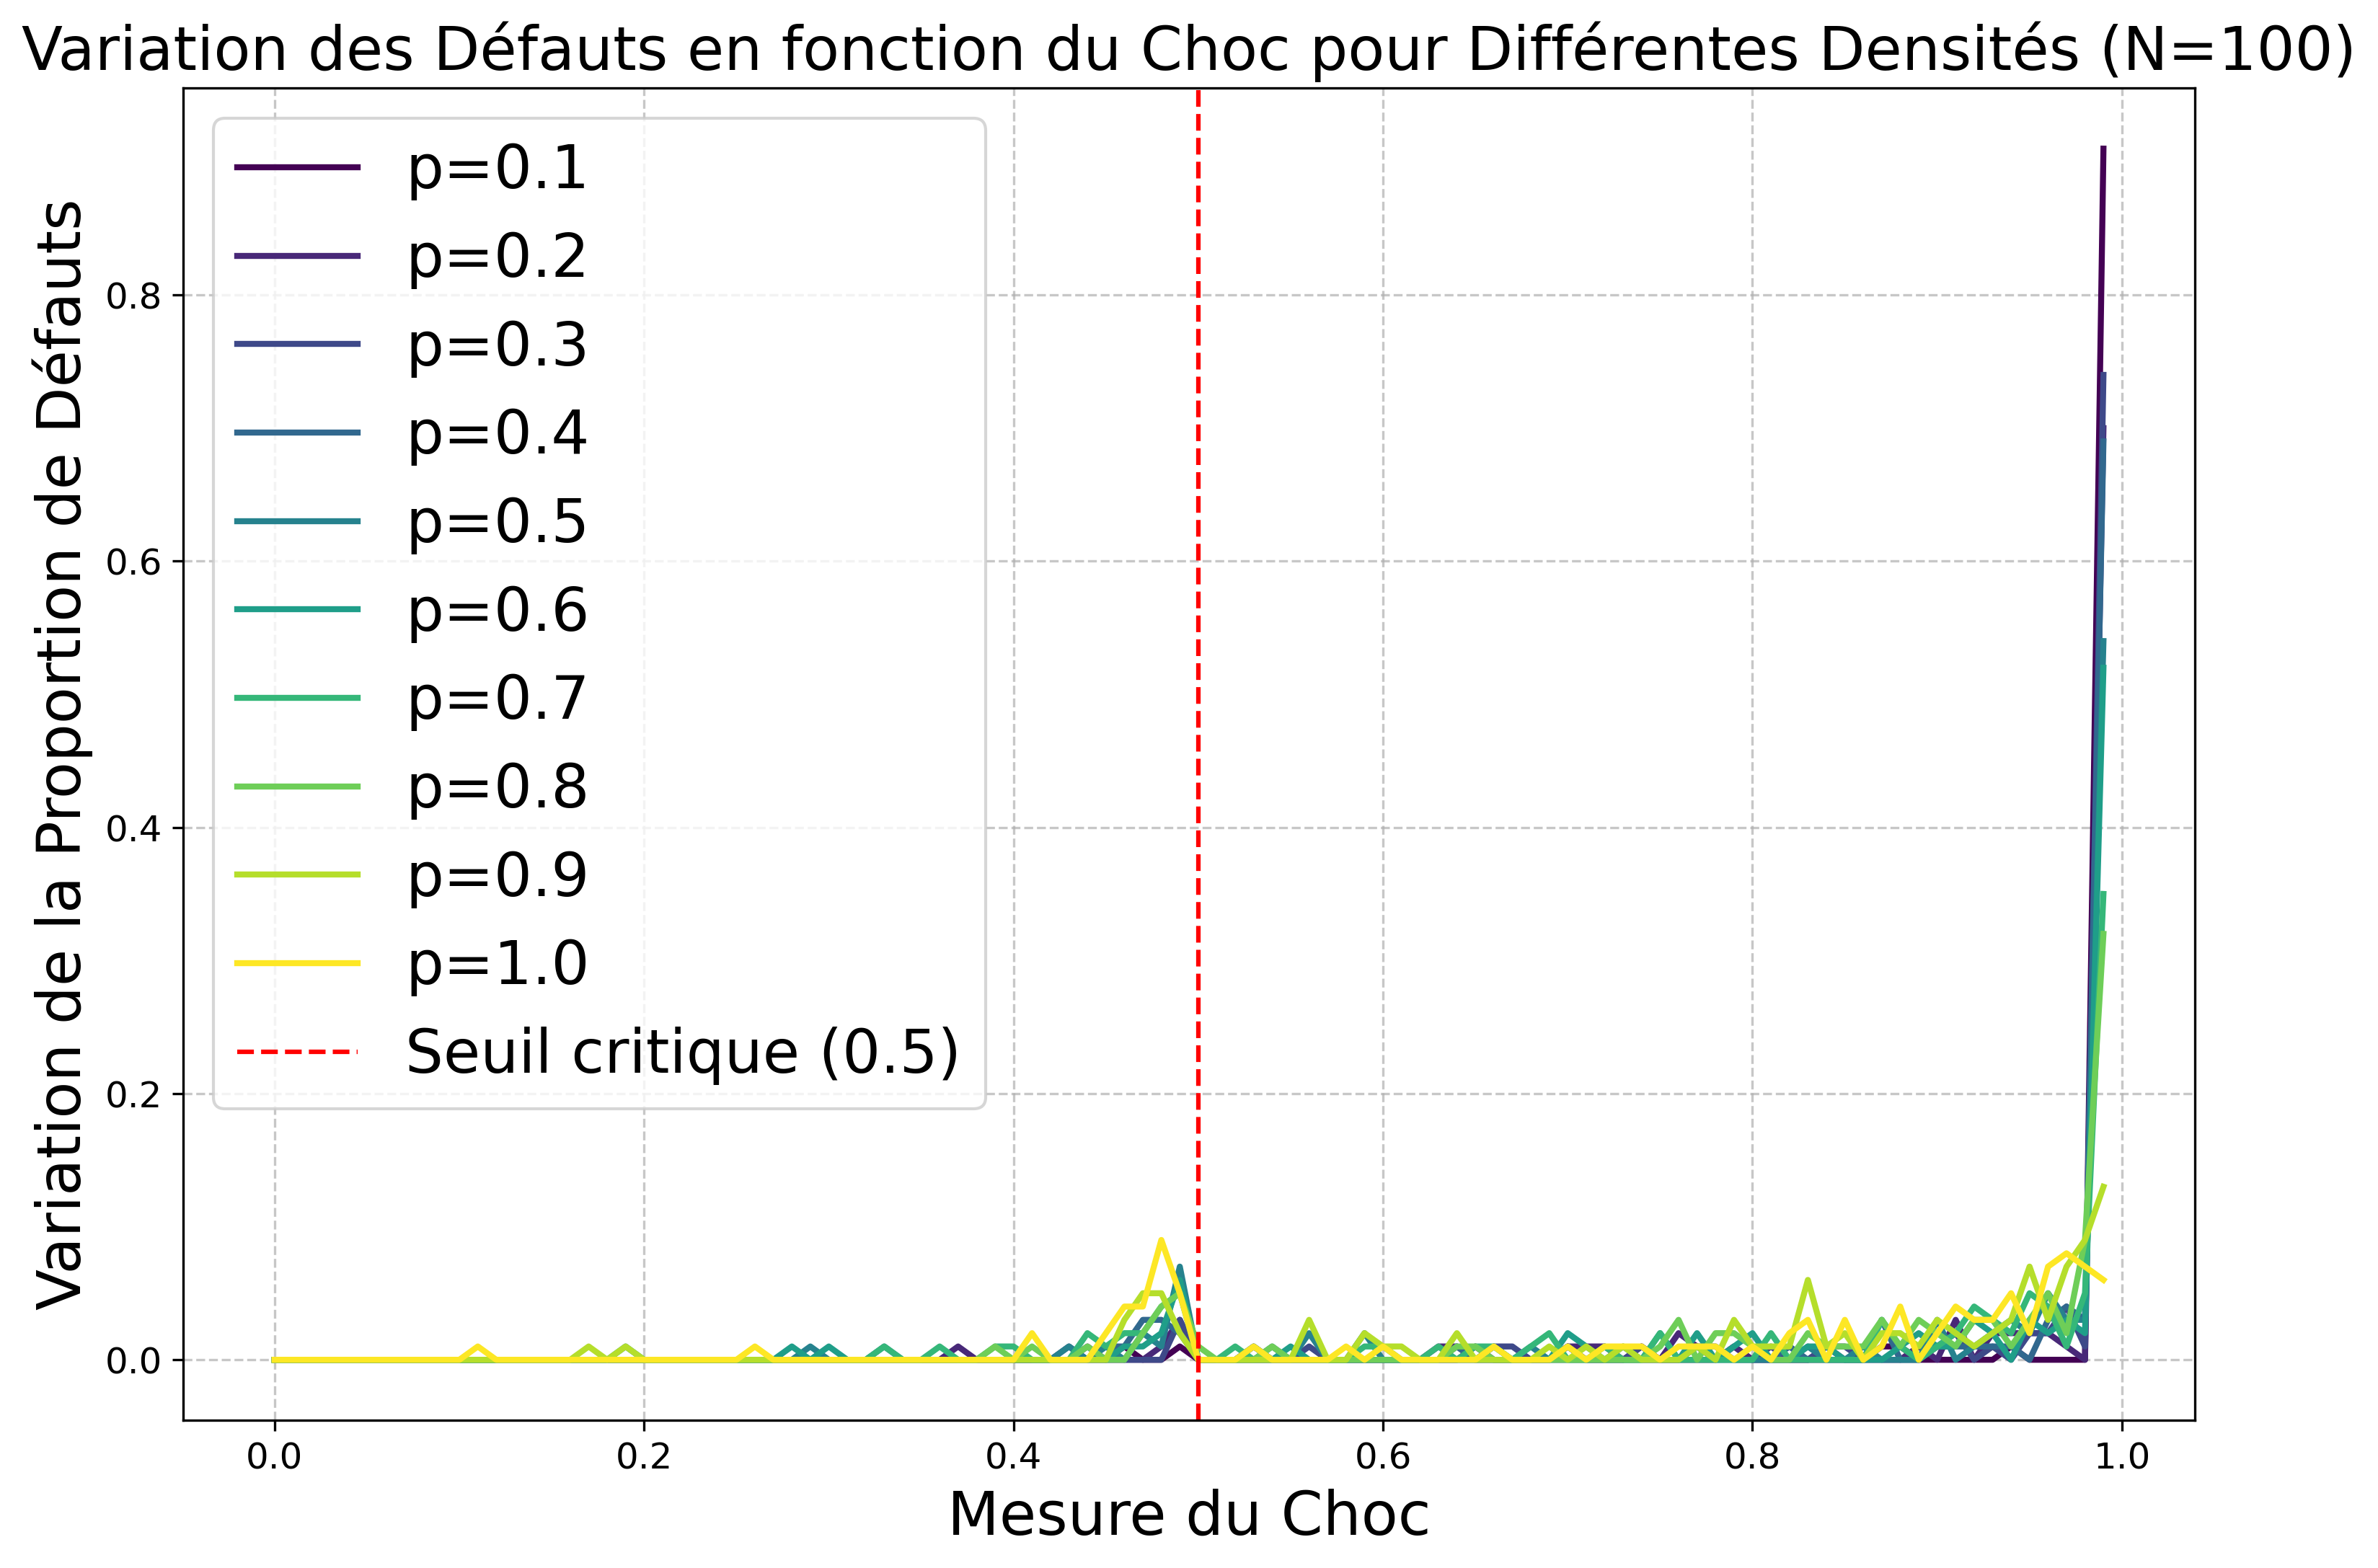
\includegraphics[width=\columnwidth]{fig4_2d_variation_shock_default.png}
    \caption{Variation de la proportion de défauts en fonction de la mesure du choc, mettant en évidence le pic autour de la valeur critique de 0.5.}
    \label{fig:variation_default}
\end{figure}

\subsection{Hypothèses d'interprétation}\label{subsec:hypotheses-d'interpretation}

Si l'on compare ce phénomène avec les transitions de phase classiques dans les graphes d'Erdős-Rényi, on constate une différence fondamentale : alors que la théorie établie des graphes aléatoires s'intéresse à l'émergence d'une composante géante en fonction de la probabilité de connexion ($p \approx 1/N$), notre observation concerne un seuil critique par rapport à l'amplitude du choc exogène.

Plusieurs hypothèses peuvent être avancées pour tenter d'expliquer ce phénomène :

\begin{enumerate}
    \item \textbf{Avant le seuil critique} : Les défauts pourraient rester relativement contenus car le système dispose de suffisamment de capital pour absorber partiellement le choc.

    \item \textbf{Au voisinage du seuil} : Le réseau pourrait atteindre un point où les banques les plus vulnérables font défaut simultanément, créant un effet d'amplification temporaire.

    \item \textbf{Après le seuil} : Le système semble se restabiliser, peut-être parce que les banques les plus fragiles ayant déjà fait défaut, les banques restantes sont plus résilientes face à l'augmentation continue du choc.
\end{enumerate}

Il est important de noter que ces hypothèses restent à vérifier par des analyses plus approfondies et ne constituent pas des conclusions définitives.

\subsection{Influence de la densité du réseau}\label{subsec:influence-de-la-densite-du-reseau}

Notre étude visait initialement à déterminer l'influence de la densité du réseau sur sa résilience face aux chocs. La Figure \ref{fig:3d_density_shock} présente la relation entre la probabilité de connexion, l'amplitude du choc, et la proportion de défauts.

\begin{figure}[htbp]
    \centering
    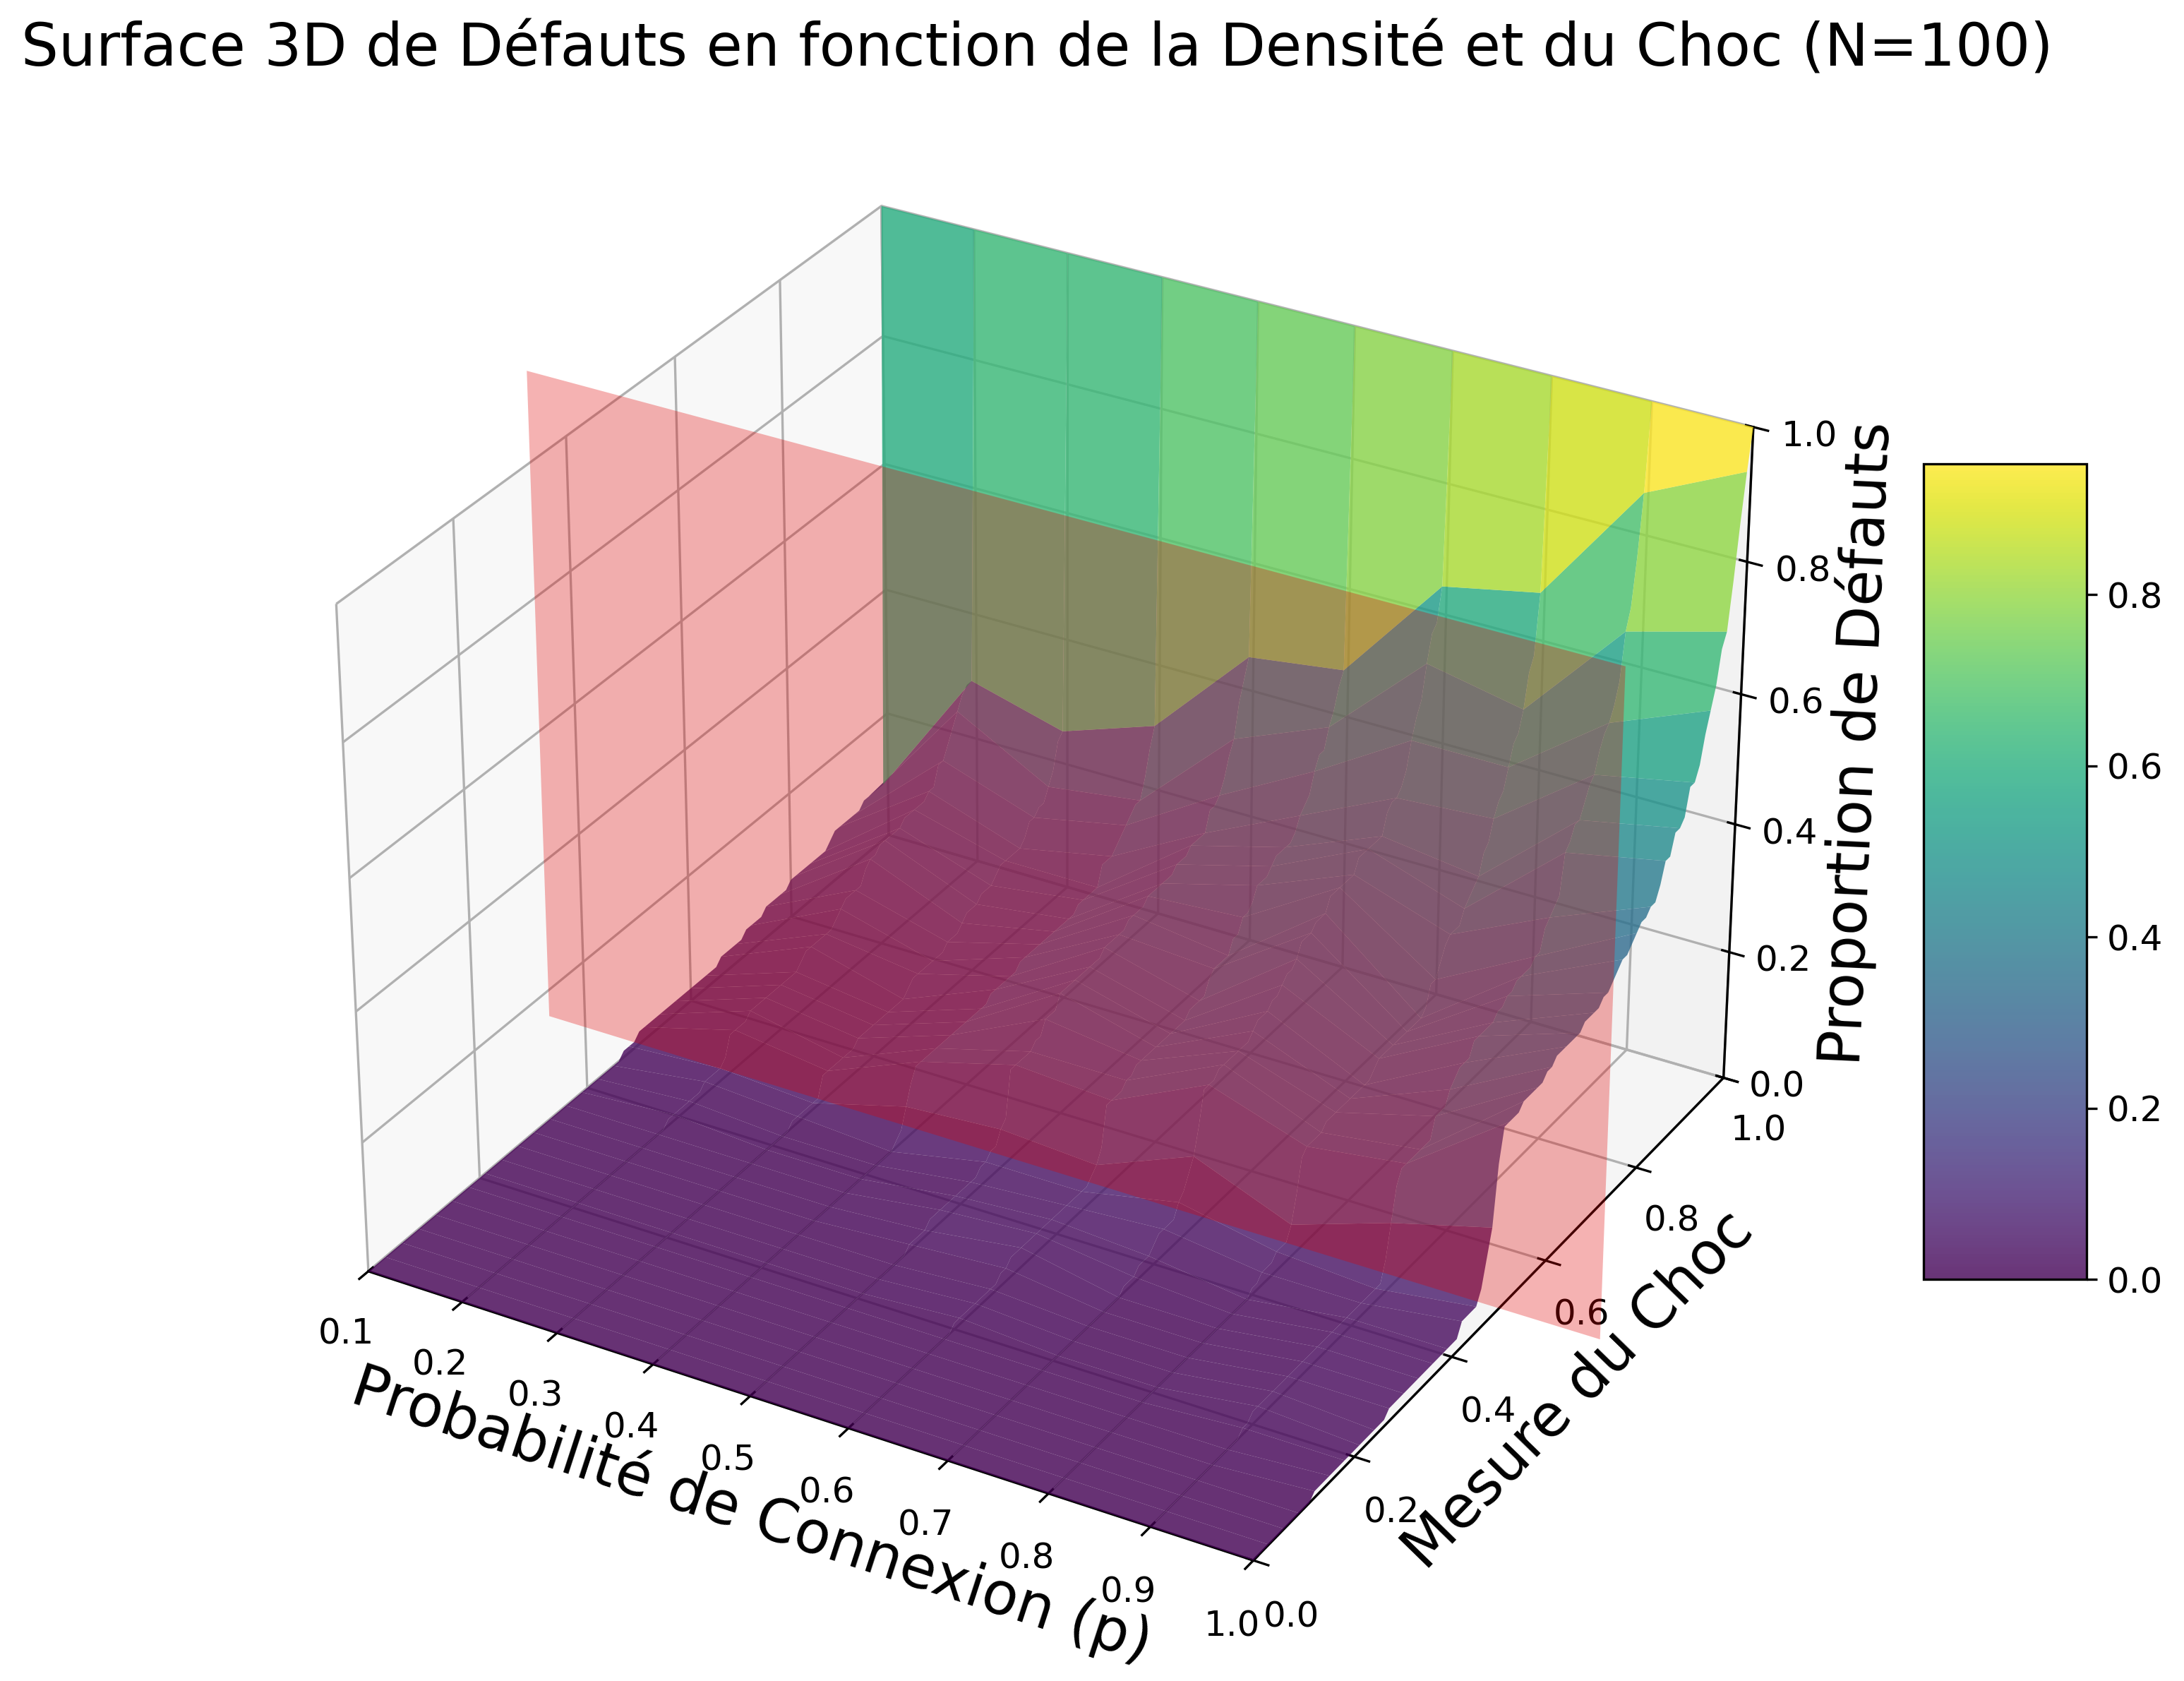
\includegraphics[width=\columnwidth]{fig3_3d_prob_shock_default.png}
    \caption{Surface 3D illustrant la relation entre la densité du réseau, l'amplitude du choc et la proportion de défauts résultante.}
    \label{fig:3d_density_shock}
\end{figure}

L'analyse de cette visualisation révèle un résultat contre-intuitif : les réseaux moins connectés apparaissent plus résistants aux chocs que les réseaux densément connectés. Ce constat va à l'encontre de l'hypothèse de diversification du risque défendue par \cite{peyton2016contagion}, selon laquelle une plus grande interconnexion devrait permettre de mieux diluer l'impact des chocs.

\subsection{Effet de l'échelle du réseau}\label{subsec:effet-de-l'echelle-du-reseau}

Nous avons également examiné l'influence du nombre de banques sur la dynamique de propagation des défauts, comme illustré dans la Figure \ref{fig:3d_banks_shock}.

\begin{figure}[htbp]
    \centering
    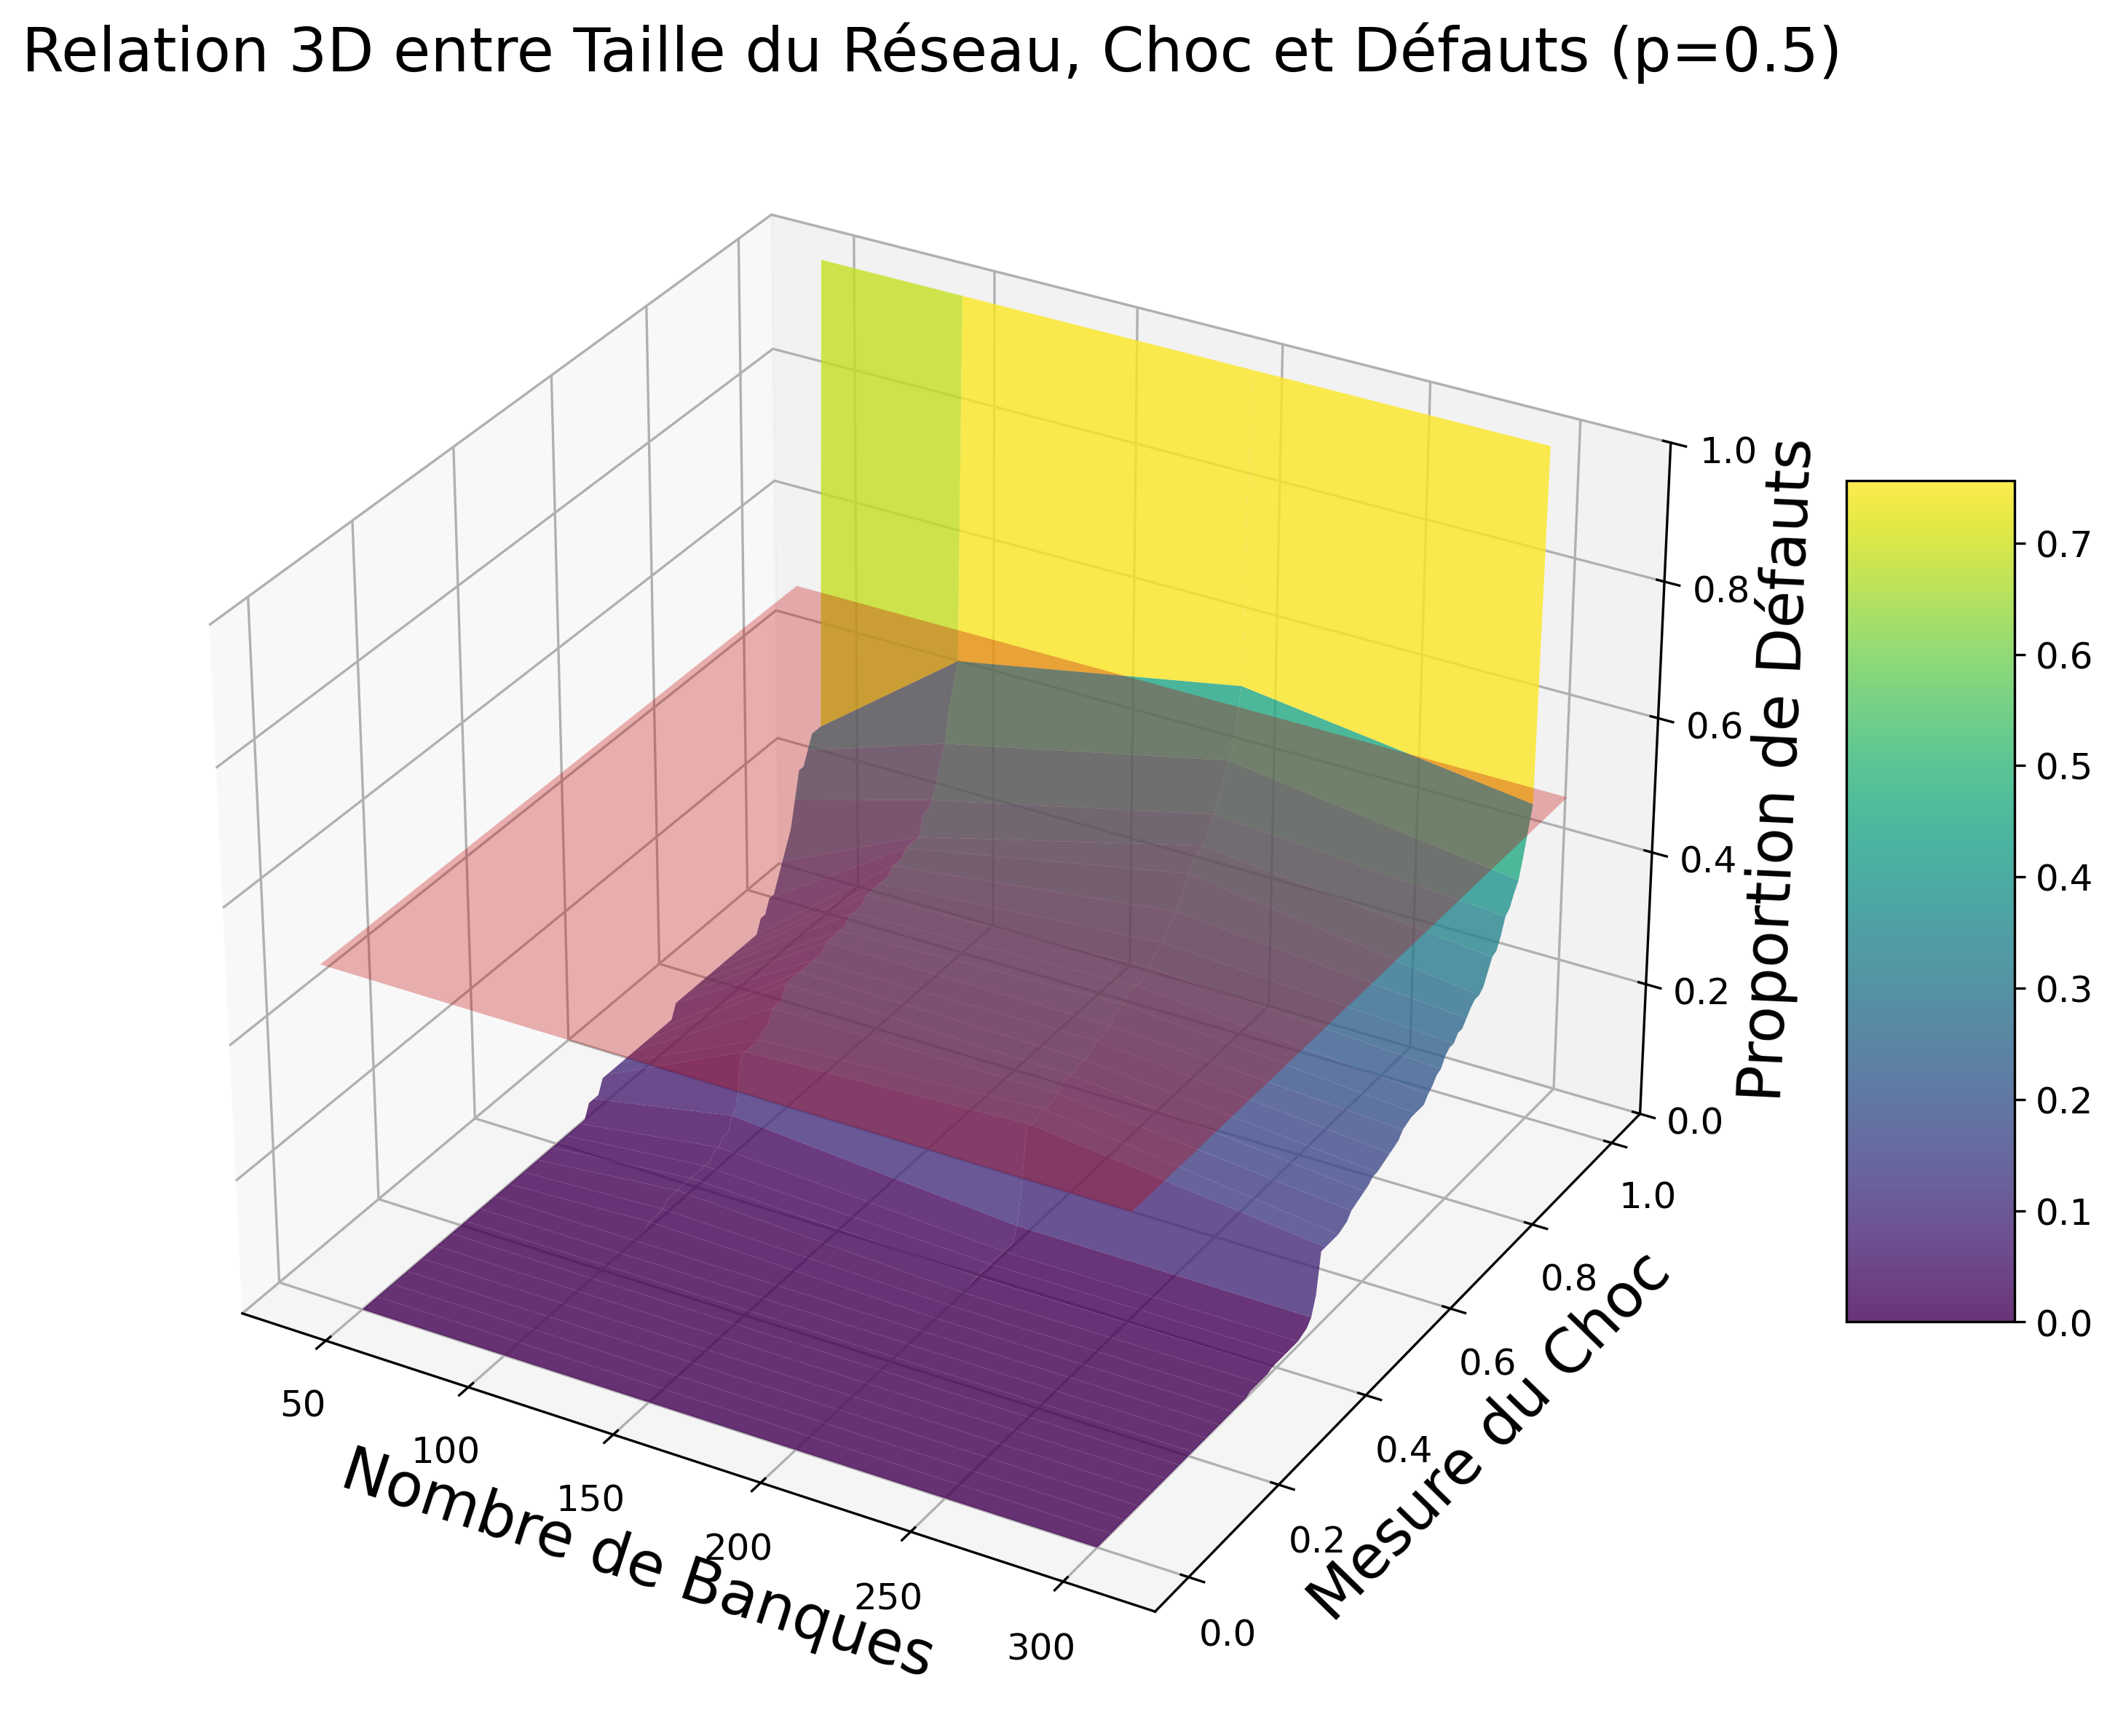
\includegraphics[width=\columnwidth]{fig1_3d_bank_shock_default.png}
    \caption{Surface 3D illustrant la relation entre le nombre de banques, l'amplitude du choc et la proportion de défauts résultante pour une probabilité de connexion fixée à 0.5.}
    \label{fig:3d_banks_shock}
\end{figure}

Ce graphique confirme la persistance du seuil critique autour de $S \approx 0.5$ indépendamment de la taille du réseau, renforçant l'hypothèse d'une propriété structurelle plutôt que d'un artefact lié à l'échelle du système.

\subsection{Limites de l'approche actuelle}\label{subsec:limites-de-l'approche-actuelle}

Notre analyse présente plusieurs limites qui doivent être soulignées :

\begin{enumerate}
    \item \textbf{Difficulté à isoler l'effet de diversification} : Notre modèle actuel, basé sur des chocs exogènes proportionnels aux actifs extérieurs, ne permet pas de distinguer clairement entre l'effet de dilution du risque par la diversification et l'effet du simple volume de capital.

    \item \textbf{Résultats contre-intuitifs sur la densité} : Nos graphiques 3D suggèrent que les réseaux moins connectés seraient plus résistants, ce qui va à l'encontre de l'intuition financière sur les bénéfices de la diversification.

    \item \textbf{Complexité des mécanismes sous-jacents} : L'identification d'un seuil à 0.5 est intrigante mais pourrait résulter de la structure particulière de notre modèle plutôt que d'une propriété fondamentale des réseaux financiers.
\end{enumerate}

Ces visualisations illustrent bien les limites de notre approche actuelle, qui ne permet pas encore de répondre clairement à notre question initiale sur le rôle bénéfique ou néfaste des interconnexions dans la résilience du système.

Le phénomène de seuil observé mérite d'être approfondi par d'autres analyses.
Plusieurs pistes pourraient être explorées, ce qu'on verra dans les perspectives ~\ref{subsec:developpements-futurs}.